\documentclass[10pt]{beamer}
\usepackage{beamerthemeshadow}
\usepackage{graphicx}
\usepackage{color}
\usepackage[utf8]{inputenc}
\usepackage{hyperref}
\usepackage{makecell}               

\usepackage[english, serbian]{babel}        

\definecolor{}{rgb}{0.5, 0.3, 0.6}
\setbeamercolor{structure}{}

\title{Tehničko i naučno pisanje}
\subtitle{-- Roboti kao nastavnici --}
\author{Jovan Mijajlović, Miona Sretenović,\\ Mina Protić, Mihailo Marković}
\institute{Matematički fakultet\\Univerzitet u Beogradu}
\date{
	\footnotesize{Beograd, 2022.}	
}

\begin{document}
\begin{frame}
	\thispagestyle{empty}
	\titlepage
\end{frame}

\addtocounter{framenumber}{-1}

\begin{frame}[fragile]\frametitle{Sadržaj}
	\tableofcontents[]
\end{frame}

\section{Roboti kao nastavnici}

\subsection{Implementacija tehnologije u nastavi}

\begin{frame}[fragile]\frametitle{Implementacija tehnologije u nastavi}
	\begin{itemize}
	\item Razvoj tehnologije i njen uticaj
	\item Potreba za digitalnim opismenjavanjem
    \item Uvođenje onlajn nastave
    \item Informatika kao obavezan predmet
	\end{itemize}
\end{frame}

\subsection{Nastavnici}

\begin{frame}[fragile]\frametitle{Nastavnici - uloga i značaj u nastavi}
	\begin{itemize}	
        \item Uloga nastavnika
        \item Entuzijazam
        \item Komunikacija i rad
        \item Šta se očekuje od nastavnika?
        \begin{figure}[h!]
        \centering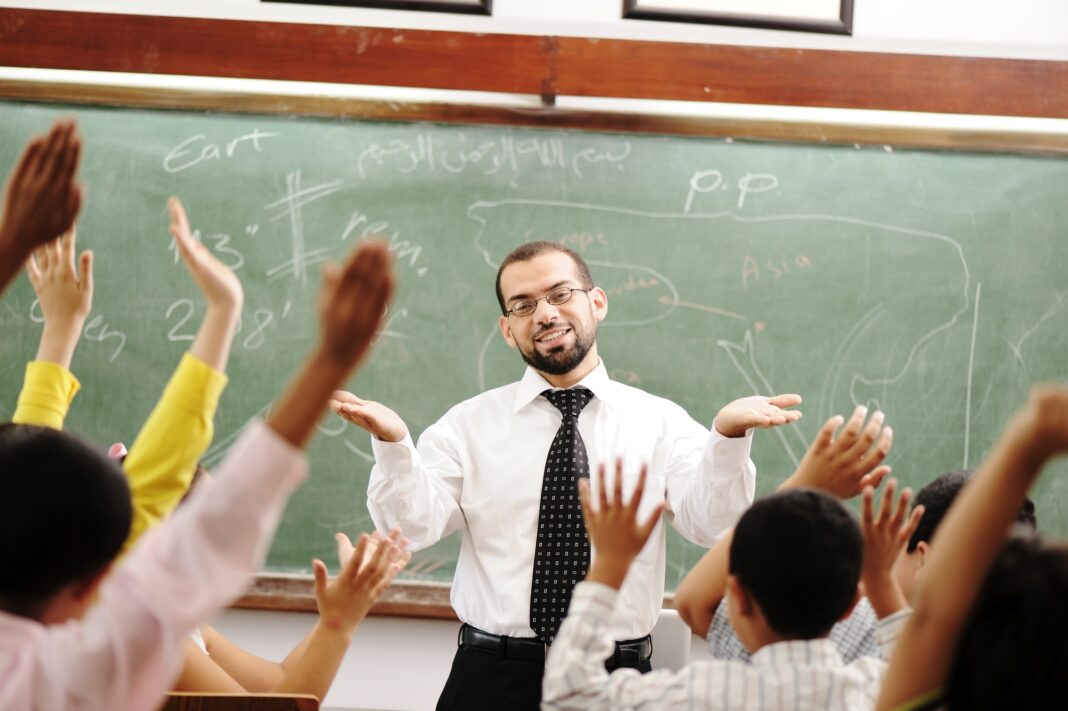
\includegraphics[height=3cm]{nastavnik.jpg} 
        \caption{Nastavnik}
        \label{fig:nastavnik}
        \end{figure}
 \end{itemize}
\end{frame}

\subsection{Roboti}
\begin{frame}[fragile]\frametitle{Roboti}
	\begin{itemize}	
        \item Šta je robot?
        \item Kako robot razmišlja?
        \item Vrste robota
    \end{itemize}

    \begin{figure}[h!]
        \centering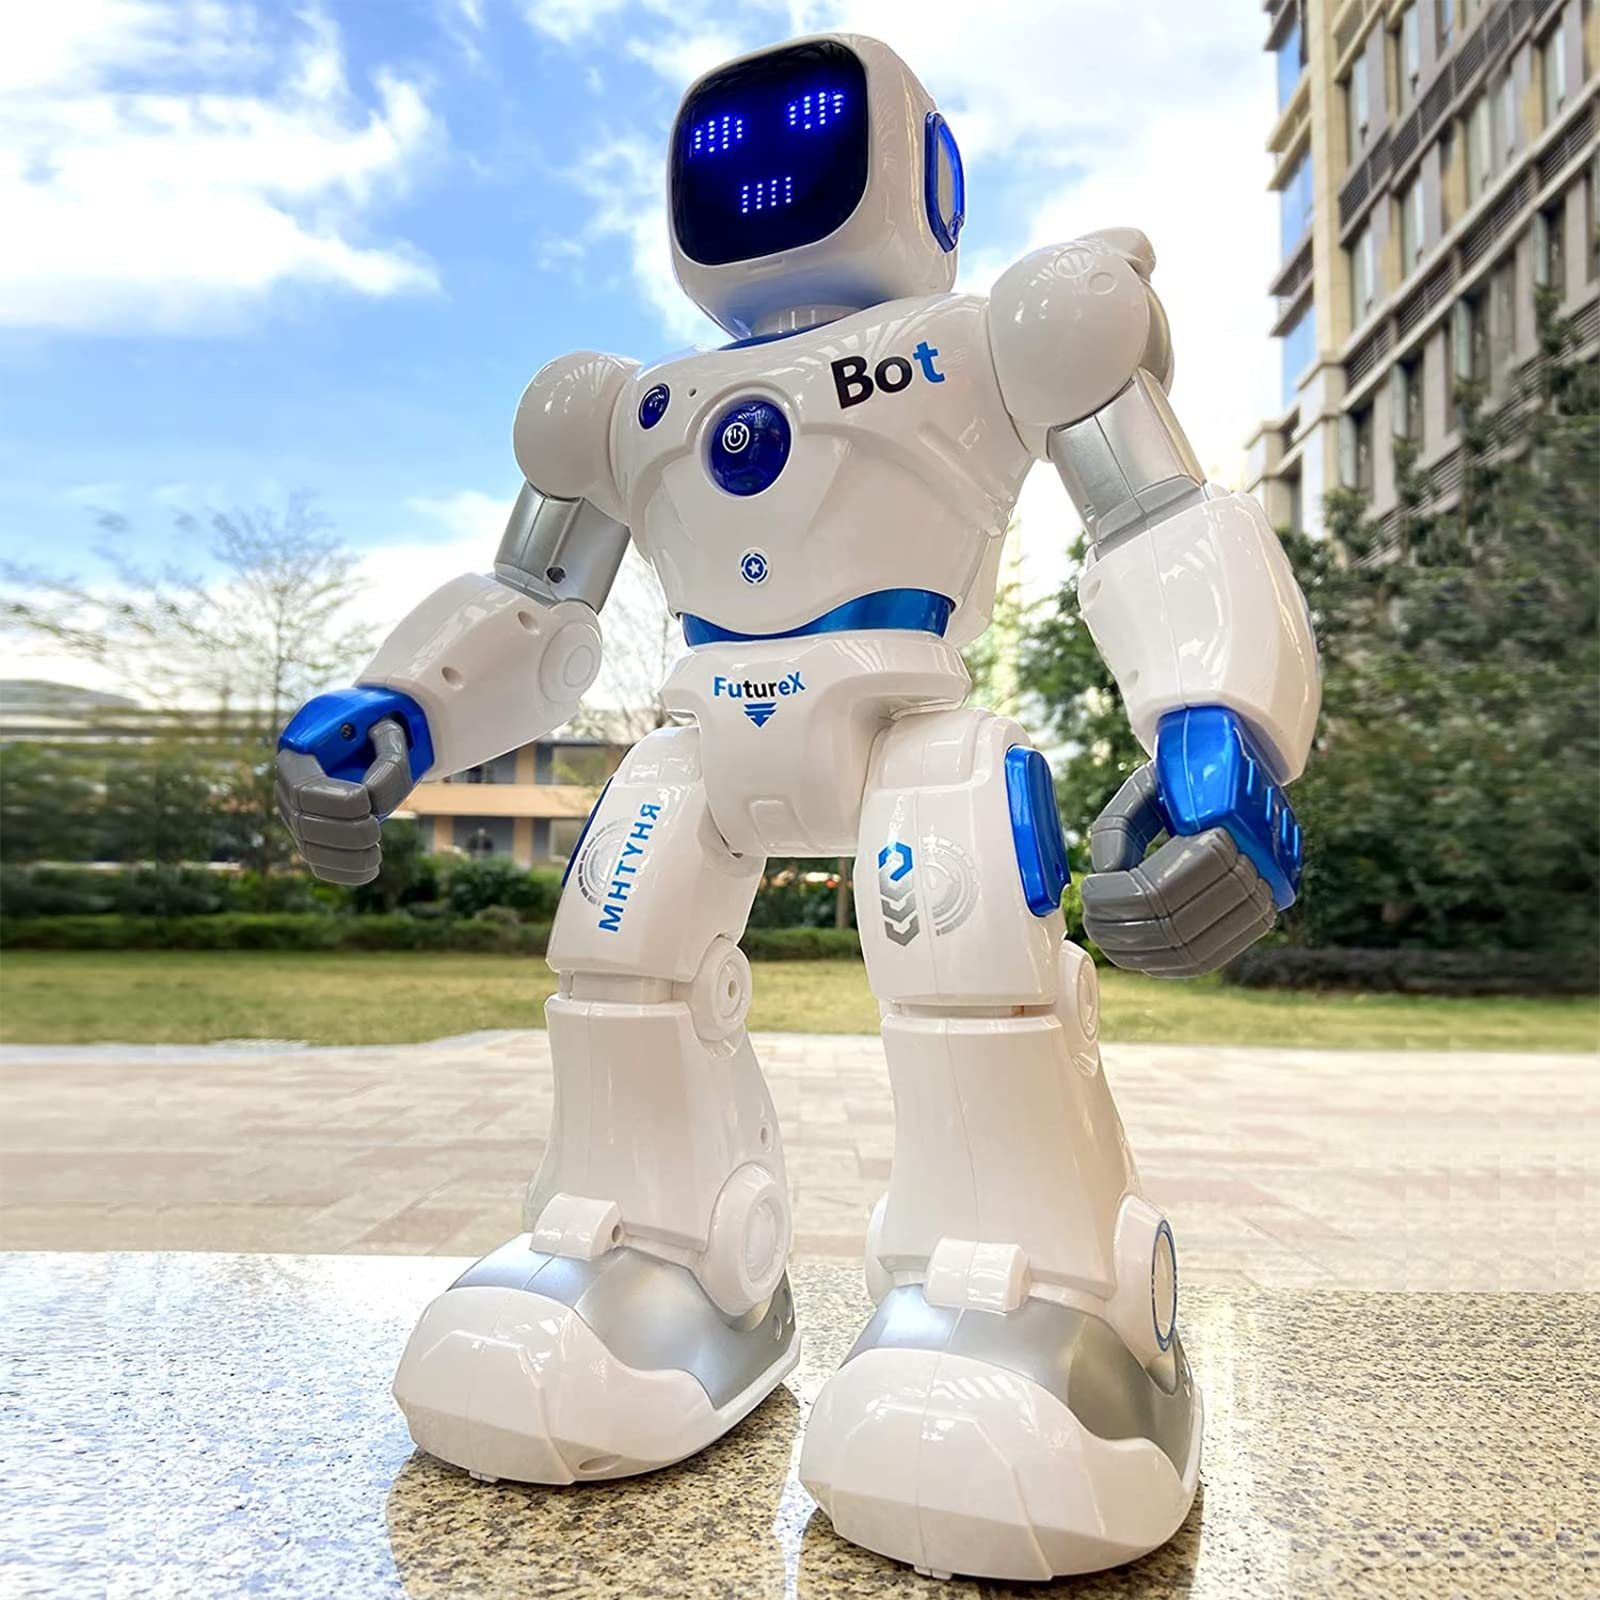
\includegraphics[height=3cm]{robot1.jpg} 
        \caption{Robot}
        \label{fig:robot}
        \end{figure}

\end{frame}

\begin{frame}[fragile]\frametitle{Roboti}
\begin{table}[ht!]
\begin{center}
\caption{Humanoidni roboti}
\begin{tabular}{|c|c|} \hline
\textbf{Ime robota}& \textbf{Opis robota}\\ \hline
Bina48 &Robot student i predavač\\ \hline
Osmo Awibe &Uz njega deca razvijaju motoričke veštine\\ \hline
Ultimate 2.0 &Napredni programabilni robotski komplet\\ \hline
Miro &Baziran na veštačkoj inteligenciji i senzorima\\ \hline
mBot &STEM robot za kodiranje\\ \hline
Jimu &Zahvaljujući njemu učenici razvijaju ljubav prema robotima\\ \hline
\end{tabular}
\label{tab:tabela1}
\end{center}
\end{table}
\end{frame}

\subsection{Primena robota}
\begin{frame}[fragile]\frametitle{Primena robota u nastavi}

\begin{itemize}
    \item Primena robota:
    \begin{itemize}
        \item Robot nastavnik
        \item Robot student
        \item Sredstvo za rad
    \end{itemize}
    \begin{figure}[h!]
        \centering\includegraphics[height=3cm]{robot_nastavnik.jpg} 
        \caption{Robot nastavnik}
        \label{fig:robotnastavnik}
        \end{figure}
    
\end{itemize}
\end{frame}

\begin{frame}[fragile]\frametitle{Bina48}
	\begin{itemize}	
        \item Bina Rothblatt
        \item Projekat LifeNaut
        \item Prvi robot nastavnik
        \begin{figure}[h!]
        \centering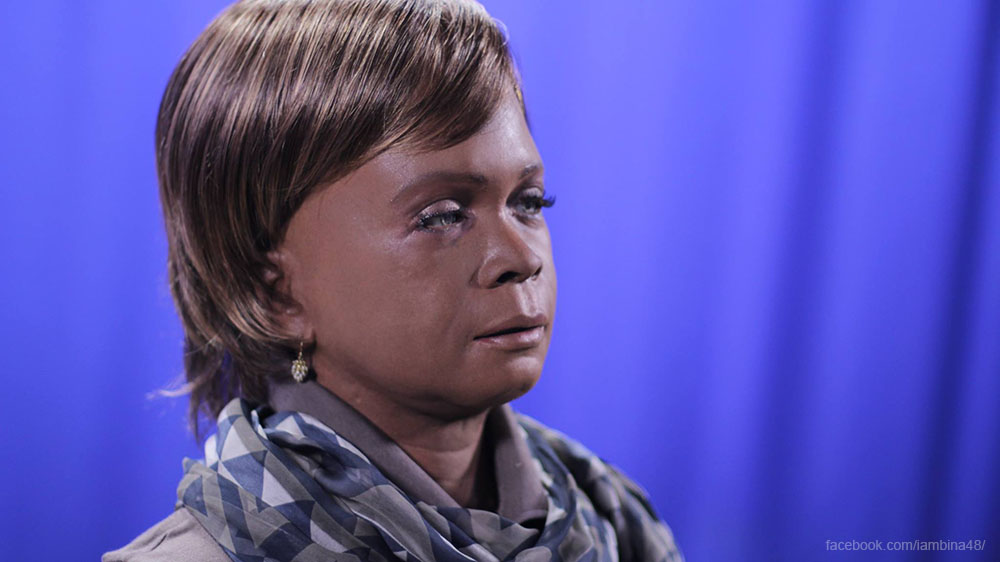
\includegraphics[height=3cm]{Bina48.jpg} 
        \caption{Bina48}
        \label{fig:bina48}
        \end{figure}
 \end{itemize}
\end{frame}

\section{Zaključak}
\begin{frame}[fragile]\frametitle{Zaključak}
	\begin{itemize}	
        \item Uključenje robota u nastavu je korisno, možda čak i neizbežno zbog razvoja savremenih tehnologija.
        \item Roboti neće moći u potpunosti da zamene nastavnike, zbog emocionalne interakcije koja ne može biti zamenjena veštačkom inteligencijom.
        \item Za ovakav vid učenja, neophodan je veliki broj istraživanja, ali i ulaganja.
 \end{itemize}
\end{frame}

\section{Literatura}
\begin{frame}[fragile]\frametitle{Literatura}
      \begin{itemize}	
            \scriptsize \item  Wikipedia, https://sr.wikipedia.org/wiki/Робот
            \scriptsize \item https://www.rts.rs/page/magazine/sr/story/1882/tehnologija/2642727/roboti-stizu-u-skolske-klupe.html
            \scriptsize \item  https://learnenglish.britishcouncil.org/skills/reading/b1-reading/robot-teachers
            \scriptsize \item  https://frontcore.com/blog/meet-the-first-robot-who-teaches-a-college-course/
            \scriptsize \item https://www.festo.com/rs/sr/e/casopis/gospodin-i-gospoda-roboti-kao-nastavnici-id\_35076/
            \scriptsize \item https://www.oberlo.com/blog/online-teaching
            \scriptsize \item{Nastavik-}Dostupno na adresi: https://www.biznisipravo.rs/kako-se-zaposljavaju-nastavnici-u-skolama/
            \scriptsize \item{Robot-}Dostupno na adresi: https://www.amazon.com/Ruko-Programmable-Interactive-Control-Present/dp/B085WPHTHW
            \scriptsize \item{Tabela -}Tabela napravljena uz pomoć sajta: https://www.savremena-osnovna.edu.rs/robot-pepper-stvarno-drugaciji-nastavnik-u-savremenoj/
	\end{itemize}
\end{frame}

\end{document}
